\section{The Chainsewing Attack}\label{sec:attack}
We now make the critical observation that a thorny block can include interlink
pointers to blocks that are not its own ancestors in the $0$-level chain.
Because it must contain a pointer to the hash of the block it points to, they
must be older blocks, but they may belong to a
different $0$-level chain. This is shown in Figure~\ref{fig:false_interlink}.

\begin{figure}
	\begin{center}
		\iftwocolumn
			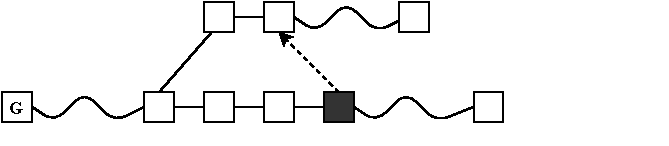
\includegraphics[width=0.6\columnwidth]{figures/false_interlink.pdf}
		\else
			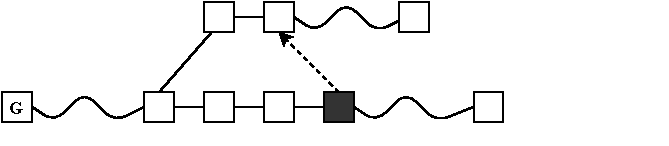
\includegraphics[width=0.35\columnwidth]{figures/false_interlink.pdf}
		\fi
	\end{center}
    \caption{A thorny block, colored black, in an honest party's chain, uses its interlink to point to a fork chain.}
	\label{fig:false_interlink}
\end{figure}

In fact, as the interlink vector contains multiple pointers, each pointer may
belong to a different fork. This is illustrated in
Figure~\ref{fig:thorny_block}. The interlink pointing to arbitrary directions
resembles a thorny bush.

\begin{figure}
	\begin{center}
		\iftwocolumn
			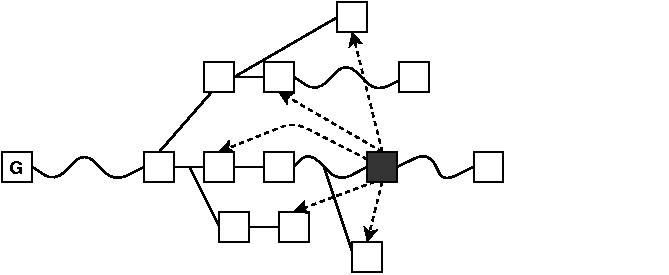
\includegraphics[width=0.5\columnwidth]{figures/thorny_block.pdf}
		\else
			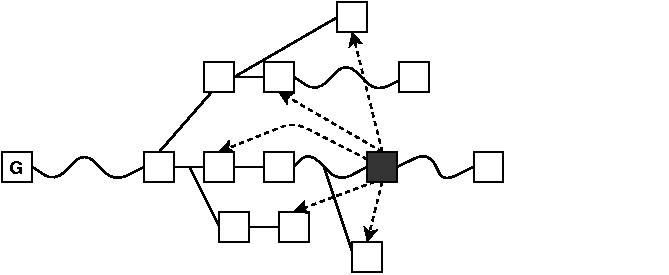
\includegraphics[width=0.4\columnwidth]{figures/thorny_block.pdf}
		\fi
	\end{center}
	\caption{A thorny block appended to an honest party's chain.
	The dashed arrows are interlink pointers.}
	\label{fig:thorny_block}
\end{figure}

We now present the \emph{chainsewing attack} against the na\"ive velvet NIPoPoW
protocol. The attack leverages thorny blocks in order to enable the adversary to
\emph{usurp} blocks belonging to a different chain and claim it as her own.
Taking advantage of thorny blocks, the adversary produces suffix proofs
containing an arbitrary number of blocks belonging to several fork chains. The
attack works as follows.

Let $\chain_B$ be a chain adopted by an honest party $B$ and $\chain_\mathcal{A}$, a fork of $\chain_B$ at some point, be maintained by the adversary. After the fork point $b = (\chain_B \cap \chain_\mathcal{A})[-1]$, the honest party produces a block extending $b$ in $\chain_B$ containing a transaction $\tx$. The adversary includes a conflicting (double spending) transaction $\tx'$ in a block extending $b$ in $\chain_\mathcal{A}$.
The adversary produces a suffix proof to convince the verifier that $\chain_\mathcal{A}$ is longer. In order to achieve this, the adversary needs to include a greater amount of total proof-of-work in her suffix proof, $\pi_\mathcal{A}$, in comparison to that included in the honest party's proof, $\pi_B$, so as to achieve $\pi_\mathcal{A} \geq_m \pi_B$. Towards this purpose, she miners intermittently on both $\chain_B$ and $\chain_\mathcal{A}$. She produces some thorny blocks in both chains $\chain_\mathcal{A}$ and $\chain_B$ which will allow her to usurp selected blocks of $\chain_B$ and present them to the light client as if they belonged to $\chain_\mathcal{A}$ in her suffix proof.

The general form of this attack for an adversary sewing blocks to one forked chain is illustrated in Figure~\ref{fig:generic_attack}. Dashed arrows represent interlink pointers of some level $\mu_\mathcal{A}$. Starting from a thorny block in the adversary's forked chain and following the interlink pointers, jumping between $\chain_\mathcal{A}$ and $\chain_B$, a chain of blocks crossing forks is formed, which the adversary claims as part of her suffix proof. Blocks of both chains are included in this proof and a verifier cannot distinguish the non-smooth pointers participating in this proof chain and, as a result, considers it a valid proof. Importantly, the adversary must ensure that any blocks usurped from the honest chain are not included in the honest NIPoPoW to force the NIPoPoW verifier to consider an earlier LCA block $b$; otherwise, the adversary will compete after a later fork point, negating any sewing benefits.

\begin{figure}
	\begin{center}
		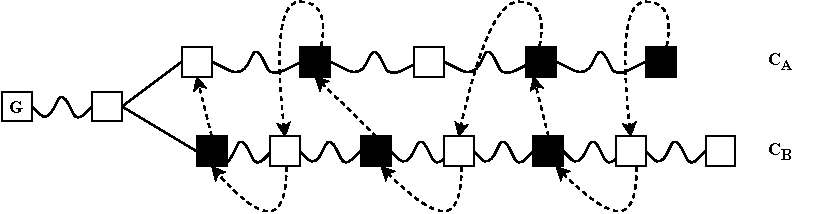
\includegraphics[width=0.9\columnwidth
		]{figures/generic_chainsewing_attack.pdf}
	\end{center}
	\caption{Generic Chainsewing Attack. $\chain_B$ is the chain of an honest party and $\chain_\mathcal{A}$ the adversary's chain. Thorny blocks are colored black. Dashed arrows represent interlink pointers included in the	adversary's suffix proof. Wavy lines imply one or more blocks.}
	\label{fig:generic_attack}
\end{figure}

This generic attack is made concrete as follows.
The adversary chooses to attack at some level $\mu_\mathcal{A} \in \mathbb{N}$ (ideally, if the honest verifier does not impose any succinctness limits, the adversary sets $\mu_A = 0$). As shown in Figure~\ref{fig:attack}, she first generates a block $b'$ in her forked chain $\chain_\mathcal{A}$ containing the double spend, and a block $a'$ in the honest chain $\chain_B$ which thorny-points to $b'$. Block $a'$ will be accepted as valid in the honest chain $\chain_B$ despite the invalid interlink pointers. The adversary also chooses a desired superblock level $\mu_B \in \mathbb{N}$ that she wishes the honest party to attain. Subsequently, the adversary waits for the honest party to mine and sews any blocks mined on the honest chain that are of level below $\mu_B$. However, she must bypass blocks that she thinks the honest party will include in their final NIPoPoW, which are of level $\mu_B$ (the blue block designated $c$ in Figure~\ref{fig:attack}). To bypass a block, the adversary mines her own thorny block $d$ on top of the current honest tip (which could be equal to the block to be bypassed, or have progressed further), containing a thorny pointer to the block preceding the block to be bypassed and hoping $d$ will not exceed level $\mu_B$ (if it exceeds that level, she discards her $d$ block). Once $m$ blocks of level $\mu_B$ have been bypassed in this manner, the adversary starts bypassing blocks of level $\mu_B - 1$, because the honest NIPoPoW will start including lower-level blocks. The adversary continues descending in levels until a sufficiently low level $\min\mu_B$ has been reached at which point it becomes uneconomical for the adversary to continue bypassing blocks (typically for a $1/4$ adversary, $\min\mu_B = 2$). At this point, the adversary forks off of the last sewed honest block. This last honest block will be used as the last block of the adversarial $\pi$ part of the NIPoPoW proof. She then independently mines a $k$-long suffix for the $\chi$ portion and creates her NIPoPoW $\pi \chi$. Lastly, she waits for enough time to pass so that the honest party's chain progresses sufficiently to make the previous bypassing guesses correct and so that no blocks in the honest NIPoPoWs coincide with blocks that have not been bypassed. This requires to wait for the following blocks to appear in the honest chain: $2m$ blocks of level $\mu_B$; after the $m^\text{th}$ $\mu_B$-level block, a further $2m$ blocks of level $\mu_B - 1$; after the $m^\text{th}$ such block, a further $2m$ blocks of the level $\mu_B - 2$, and so on until level $0$ is reached.

\begin{figure}
	\begin{center}
		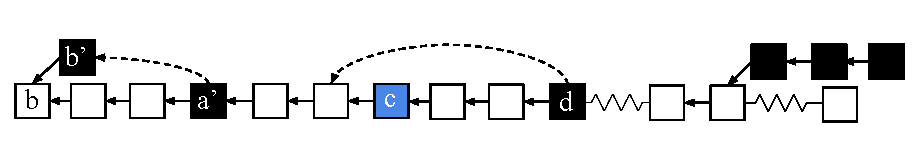
\includegraphics[width=0.99\columnwidth]{figures/chainsew-concrete.pdf}
	\end{center}
	\caption{A portion of the concrete Chainsewing Attack. The adversary's blocks are shown in black, while the honestly generated blocks are shown in white. Block $b'$ contains a double spend, while block $a'$ sews it in place. The blue block $c$ is a block included in the honest NIPoPoW, but it is bypassed by the adversary by introducing block $d$ which, while part of the honest chain, points to $c$'s parent. After a point, the adversary forks off and creates $k = 3$ of their own blocks.}
	\label{fig:attack}
\end{figure}

In this attack the adversary uses thorny blocks to ``sew'' portions of the
honestly adopted chain to her own forked chain. This justifies the name given to
the attack.
In order to make this attack successful, the adversary needs only to
produce few superblocks, while she can arrogate a large number of
honestly produced blocks. 
%Thus the attack succeeds with non-negligible probability.

We believe that the superlight-client protocol FlyClient\cite{flyclient} is also susceptible to Chainswewing attack under velvet fork conditions. 
We give insight for the velvet FlyClient attack in Appendix~\ref{sec:flyclient}.

%We illustrate simulation results for the success rate of our attack in Appendix~\ref{sec:simulation}. Our experiments find the attack with parameters $\mu_B = 10, \mu_A = 0, t = 1, n = 5, k = 15$ succeeds with a constant rate of success of approximately $0.26$, when the security parameter $m$ ranges from $3$ to $15$. This is in contrast to the best previously known attack (which does not make use of thorny blocks), which succeeds with probability less than $0.01$. Previous work recommends $m = 15$ for a $1/3$ adversary for a probability of failure bounded by $0.001$.
